% For double-blind review submission, w/o CCS and ACM Reference (max submission space)
\documentclass[sigplan,10pt,review,anonymous]{acmart}\settopmatter{printfolios=true,printccs=false,printacmref=false}
%% For double-blind review submission, w/ CCS and ACM Reference
%\documentclass[sigplan,review,anonymous]{acmart}\settopmatter{printfolios=true}
%% For single-blind review submission, w/o CCS and ACM Reference (max submission space)
%\documentclass[sigplan,review]{acmart}\settopmatter{printfolios=true,printccs=false,printacmref=false}
%% For single-blind review submission, w/ CCS and ACM Reference
%\documentclass[sigplan,review]{acmart}\settopmatter{printfolios=true}
%% For final camera-ready submission, w/ required CCS and ACM Reference
%\documentclass[sigplan]{acmart}\settopmatter{}

% Use the postscript times font!
\usepackage{times}
\usepackage{soul}
\usepackage{url}
\usepackage[hidelinks]{hyperref}

\usepackage[utf8]{inputenc}
\usepackage[english]{babel}
\usepackage[small]{caption}

%%%%%%
\newtheorem{theorem}{Theorem}

% Math notation
\RequirePackage[group-separator={,}]{siunitx}
\newcommand{\na}{$\mathrm{N.A.}$}
\newcommand{\minus}{\scalebox{0.7}[1.0]{$-$}}
\newcommand{\expn}[1]{\!\!\times\!\!10^{\minus#1}}
\newcommand{\pval}[2]{$p\textrm{-value} = #1\expn{#2}$}
\newcommand{\set}[1]{\{{}#1\}}
\newcommand{\A}[1]{\mathcal{A}_{#1}}
\newcommand{\N}[1]{n_{#1}(j)}



%%%%%%
\usepackage{float}
\usepackage{listings}
\usepackage{caption}
\usepackage{graphicx}
\usepackage{subcaption}
\usepackage{colortbl}
\usepackage{amsmath}
%\usepackage{amsthm} 
\usepackage{mathpartir}
\usepackage{fancyvrb}\fvset{fontsize=\small}
\usepackage{xspace}
\usepackage{xcolor}
\usepackage{balance}
\usepackage{wrapfig}
\usepackage{multirow}
\usepackage{pifont}
\usepackage{amssymb}
%%%%%%%%%%%%%%%%%%% this can reduce space quite a lot
\usepackage{soul}
\usepackage{microtype}
\usepackage[T1]{fontenc}
\usepackage{dsfont}
%%%%%%%%%%%%%%%%%%% this can reduce space quite a lot
\usepackage{relsize}
\usepackage{tikz}
\usepackage{longtable}
\usepackage{booktabs}
\usepackage{marvosym} 
\usepackage{framed}
\usepackage{mdwlist}
\usepackage{tabularx}
\usepackage{wrapfig}

\usepackage{array}
\usepackage{mathtools}
\usepackage{url}
\usepackage{color}

%% Colors
\definecolor{bgBlock}{rgb}{0.22,0.15,0.49}
\definecolor{bgBlockAlert}{rgb}{0.99,0.84,0.31}
\definecolor{fgBlockAlert}{rgb}{0.22,0.15,0.49}
\definecolor{fgBlock}{rgb}{0.99,0.84,0.31}
\definecolor{darkred}{rgb}{0.5,0,0}
\definecolor{darkgreen}{rgb}{0,0.5,0}
\definecolor{darkblue}{rgb}{0,0,0.5}
\definecolor{Gray}{gray}{0.9}

%%%%%%%%%% added by sofia
\usepackage{algpseudocode}
\usepackage{algorithm}
\usepackage{enumitem}


\usepackage{bm}
\usepackage{cleveref}
\usepackage{textcomp}
\usepackage{pdfpages}
\usepackage{chngpage}


%\usepackage[hyphenbreaks]{breakurl}


%%%%%%%%%%

\usepackage[most]{tcolorbox}
\newtcolorbox{myframe}[1][]{
	enhanced,
	arc=0pt,
	outer arc=0pt,
	colback=white,
	boxrule=0.5pt,
	boxsep=1pt,left=3pt,right=3pt,top=5pt,bottom=5pt,
	fontupper=\small,
	size=small
	#1
}

%%%%%%%%%%
% appendix 
\usepackage[toc,page]{appendix}
\usepackage{makecell}


%%%%% Theorem -> Claim

\newtheorem{thm}{Theorem} % the main one
\newtheorem{lemma}[thm]{Lemma}

\newcommand{\thistheoremname}{}
\newtheorem{genericthm}[thm]{\thistheoremname}
\newenvironment{namedthm}[1]
  {\renewcommand{\thistheoremname}{#1}
   \begin{genericthm}}
  {\end{genericthm}}





\newcommand{\Fix}[1]{\textbf{[[}{\color{red} #1}\textbf{]]}}
\newcommand{\Anonim}[2]{#1}
\newcommand{\ie}{i.e.}
\newcommand{\eg}{e.g.}
\newcommand{\cf}{cf.}
\newcommand{\etal}{et al.}
\newcommand{\comments}[1]{}
\newcommand{\varex}{\textsc{Varex}}
\newcommand{\tsig}{OUR}
\newcommand{\tnamepar}[1]{\tname{}\texttt{[#1]}}
\newcommand{\CodeIn}[1]{{\small\texttt{#1}}}
\newcommand{\pw}{\textsc{pw}}
\newcommand{\pwopt}{\textsc{pw-opt}}
\newcommand{\dd}{\CodeIn{DD}}
\newcommand{\acrAbrev}{APR}
\newcommand{\RQ}{RQ}
\newcommand{\morpho}{\emph{morpho}}
\newcommand{\lithium}{\emph{lithium-slicer}}
\newcommand{\success}{\leavevmode\color[HTML]{009901}}

\definecolor{bs}{rgb}{0.59, 0.0, 0.09}
\definecolor{d}{HTML}{800000}

\newcommand{\BS}[1]{\textbf{[BS:[}{\color{bs} #1}\textbf{]]}}
\newcommand{\Mar}[1]{\textbf{[Marcelo:[}{\color{orange} #1}\textbf{]]}}
\newcommand{\Sof}[1]{\textbf{[Sofia:[}{\color{cyan} #1}\textbf{]]}}
\newcommand{\oururl}{\Fix{url here}}
\newcommand{\tname}{\Fix{Critical Slicing Revisited}}

\newcommand{\numPrograms}{six}
\newcommand{\numFaults}{395}
\newcommand{\topk}{top-$k$}

\newcommand{\sfl}{SFL}
\newcommand{\CS}{CS}
\newcommand{\cs}{CS}
\newcommand{\ds}{DS}
\newcommand{\dfj}{Defects4J}
\newcommand{\orbs}{ORBS}
\newcommand{\comb}{\sfl{}+\ds{}}
\newcommand{\apr}{APR}

%% subject names as in https://github.com/rjust/defects4j
\newcommand{\chart}{JFreechart}
\newcommand{\closure}{Closure compiler}
\newcommand{\lang}{Apache commons-lang}
\newcommand{\cmath}{Apache commons-math}
\newcommand{\mockito}{Mockito}
\newcommand{\jtime}{Joda-Time}

\newcommand{\cmark}{\ding{51}}%
\newcommand{\xmark}{\ding{55}}%


%% Conference information
%% Supplied to authors by publisher for camera-ready submission;
%% use defaults for review submission.
\acmConference[PLDI'19]{ ACM SIGPLAN Conference on Programming Language Design and Implementation}{June 24--26, 2019}{Phoenix, AZ, USA}
\acmYear{2019}
\acmISBN{} % \acmISBN{978-x-xxxx-xxxx-x/YY/MM}
\acmDOI{} % \acmDOI{10.1145/nnnnnnn.nnnnnnn}
\startPage{1}

%% Copyright information
%% Supplied to authors (based on authors' rights management selection;
%% see authors.acm.org) by publisher for camera-ready submission;
%% use 'none' for review submission.
\setcopyright{none}
%\setcopyright{acmcopyright}
%\setcopyright{acmlicensed}
%\setcopyright{rightsretained}
%\copyrightyear{2018}           %% If different from \acmYear

%% Bibliography style
\bibliographystyle{ACM-Reference-Format}
%% Citation style
%\citestyle{acmauthoryear}  %% For author/year citations
%\citestyle{acmnumeric}     %% For numeric citations
%\setcitestyle{nosort}      %% With 'acmnumeric', to disable automatic
                            %% sorting of references within a single citation;
                            %% e.g., \cite{Smith99,Carpenter05,Baker12}
                            %% rendered as [14,5,2] rather than [2,5,14].
%\setcitesyle{nocompress}   %% With 'acmnumeric', to disable automatic
                            %% compression of sequential references within a
                            %% single citation;
                            %% e.g., \cite{Baker12,Baker14,Baker16}
                            %% rendered as [2,3,4] rather than [2-4].

%%%%%%%%%%%%%%%%%%%%%%%%%%%%%%%%%%%%%%%%%%%%%%%%%%%%%%%%%%%%%%%%%%%%%%
%% Note: Authors migrating a paper from traditional SIGPLAN
%% proceedings format to PACMPL format must update the
%% '\documentclass' and topmatter commands above; see
%% 'acmart-pacmpl-template.tex'.
%%%%%%%%%%%%%%%%%%%%%%%%%%%%%%%%%%%%%%%%%%%%%%%%%%%%%%%%%%%%%%%%%%%%%%

\begin{document}

%% Title information
\title{Reassessing the Impact of Dynamic Slicing in SFL}         %% [Short Title] is optional;
                                        %% when present, will be used in
                                        %% header instead of Full Title.
%\titlenote{with title note}             %% \titlenote is optional;
                                        %% can be repeated if necessary;
                                        %% contents suppressed with 'anonymous'
%\subtitle{Subtitle}                     %% \subtitle is optional
%\subtitlenote{with subtitle note}       %% \subtitlenote is optional;
                                        %% can be repeated if necessary;
                                        %% contents suppressed with 'anonymous'


%% Author information
%% Contents and number of authors suppressed with 'anonymous'.
%% Each author should be introduced by \author, followed by
%% \authornote (optional), \orcid (optional), \affiliation, and
%% \email.
%% An author may have multiple affiliations and/or emails; repeat the
%% appropriate command.
%% Many elements are not rendered, but should be provided for metadata
%% extraction tools.

%% Author with single affiliation.
\author{First1 Last1}
\authornote{with author1 note}          %% \authornote is optional;
                                        %% can be repeated if necessary
\orcid{nnnn-nnnn-nnnn-nnnn}             %% \orcid is optional
\affiliation{
  \position{Position1}
  \department{Department1}              %% \department is recommended
  \institution{Institution1}            %% \institution is required
  \streetaddress{Street1 Address1}
  \city{City1}
  \state{State1}
  \postcode{Post-Code1}
  \country{Country1}                    %% \country is recommended
}
\email{first1.last1@inst1.edu}          %% \email is recommended

%% Author with two affiliations and emails.
\author{First2 Last2}
\authornote{with author2 note}          %% \authornote is optional;
                                        %% can be repeated if necessary
\orcid{nnnn-nnnn-nnnn-nnnn}             %% \orcid is optional
\affiliation{
  \position{Position2a}
  \department{Department2a}             %% \department is recommended
  \institution{Institution2a}           %% \institution is required
  \streetaddress{Street2a Address2a}
  \city{City2a}
  \state{State2a}
  \postcode{Post-Code2a}
  \country{Country2a}                   %% \country is recommended
}
\email{first2.last2@inst2a.com}         %% \email is recommended
\affiliation{
  \position{Position2b}
  \department{Department2b}             %% \department is recommended
  \institution{Institution2b}           %% \institution is required
  \streetaddress{Street3b Address2b}
  \city{City2b}
  \state{State2b}
  \postcode{Post-Code2b}
  \country{Country2b}                   %% \country is recommended
}
\email{first2.last2@inst2b.org}         %% \email is recommended


%% Abstract
%% Note: \begin{abstract}...\end{abstract} environment must come
%% before \maketitle command
\begin{abstract}
\Sof{@todo}
\end{abstract}


%% 2012 ACM Computing Classification System (CSS) concepts
%% Generate at 'http://dl.acm.org/ccs/ccs.cfm'.
\begin{CCSXML}
<ccs2012>
<concept>
<concept_id>10011007.10011006.10011008</concept_id>
<concept_desc>Software and its engineering~General programming languages</concept_desc>
<concept_significance>500</concept_significance>
</concept>
<concept>
<concept_id>10003456.10003457.10003521.10003525</concept_id>
<concept_desc>Social and professional topics~History of programming languages</concept_desc>
<concept_significance>300</concept_significance>
</concept>
</ccs2012>
\end{CCSXML}

\ccsdesc[500]{Software and its engineering~General programming languages}
\ccsdesc[300]{Social and professional topics~History of programming languages}
%% End of generated code


%% Keywords
%% comma separated list
\keywords{Slicing, Testing, Debugging}  %% \keywords are mandatory in final camera-ready submission


%% \maketitle
%% Note: \maketitle command must come after title commands, author
%% commands, abstract environment, Computing Classification System
%% environment and commands, and keywords command.
\maketitle

\section{Introduction}

%\Sof{Elaborate more on the advantages of the SFL+DS combination and how DS helps SFL being more efficient}

%% PROBLEM MOTIVATION
Software debugging is difficult. The task of locating the faulty code
(\ie{}, fault localization) is particularly challenging. For that
reason, countless automated techniques have been proposed in the past
to reduce the cost of fault localization.

Dynamic Slicing (\ds{}) and Spectrum-Based Fault Localization (\sfl{})
are two very popular techniques that use different principles to
automate debugging. Dynamic
Slicing~\cite{Agrawal:1990:DPS:93542.93576} looks for the statements
in code that influence the evaluation of the fault-revealing
assertion. Although the technique has been intensively investigated in
research, few use cases gained
notoriety---WhyLine~\cite{Ko:2008:DRA:1368088.1368130} being an
exception.  \sfl{}~\cite{7390282}, in contrast, does not try to
recover the influence region of faulty statements. It is a black-box
statistical fault localization method that computes suspiciousness
values associated with program entities (e.g., basic blocks). For
that, it uses coverage information of passing and failing test
cases. \sfl{} produces a list of program entities ranked in decreasing
order of suspiciousness. Similarly to \ds{}, \sfl{} received
tremendous attention over the years, but its applicability to support
debugging remains
questionable~\cite{ang-perez-van-deursen-rui-2017,Pearson:2017:EIF:3097368.3097441,Xie:2016:RAD:2884781.2884834}.
Despite the skepticism of the research community, \sfl{} has been
shown useful in supporting downstream analyses, such as Automated
Program Repair
(\apr{})~\cite{automatic-software-repair-survey2017,kim-etal-daghstul2017},
an increasingly popular technique that looks for fixes to buggy
statements. Tools like JAFF \cite{arcuri-2011}, Prophet
\cite{long-rinard-2016}, SemFix \cite{nguyen-qi-roychoudhury-2013},
and SPR \cite{long-rinard-2015} use \sfl{} to guide the search for
likely fixes.

%Recent \apr{} techniques use \sfl{} to guide
%the search for repairs .

%% \Fix{Revise this $\rightarrow$} Mao and Wang
%% \cite{lei-mao-dai-wang-2012} had promising results compared to \sfl{}
%% state of the art techniques, such as Tarantula [cite] and Ochiai
%% [cite], concerning the relative percentage of the code above the
%% fault. Prior work used the same measurement approach
%% \cite{santelices-jones-yu-harrold-2009,wang-cheung-chan-zhang-2009,jones-2005}.
%% However, the problem with this approach lies in the effort to find the
%% defect, as shown on Parnin and Orso's study \cite{parnin-orso-2011},
%% in which a percentage rank does not scale with the size of a
%% codebase. For example, if a fault statement is ranked on the 83rd
%% position as a result of a \sfl{} technique, the percentage rank using
%% a codebase of 8300 LOC is only 1\%, with the amount of absolute lines
%% of code to be examined not being considered.  This can result in
%% millions of lines of code to be analysed, proving that a percentage
%% rank is not a practical evaluation metric
%% \cite{ang-perez-van-deursen-rui-2017}.  \Fix{end here}

%% For example, Lei \etal{}~\cite{lei-mao-dai-wang-2012} reported a
%% reduction of 78.3\% in \emph{effort}~\cite{7927959} to analyze
%% rankings when using dynamic slicing in combination with \sfl{} versus
%% plain \sfl{}.

\ds{} and \sfl{} are complementary. Intuitively, \ds{} identifies
irrelevant parts of the code whereas \sfl{} ranks the relevant parts
of the code.  This paper reports the results of a comprehensive study
to evaluate the impact of \ds{} to improve \sfl{}. The study involves
\numFaults{} faults from \numPrograms{} programs from the Defects4J (D4J)
dataset~\cite{just-defects4j-issta2014}, which is frequently used to
evaluated fault localization research. The intuition for the \comb{}
combination is that several highly ranked statements, albeit covered
by failing executions, may be unrelated to the fault. Prior work
reported promising results in this combination~\cite{Wotawa:2010:FLB:1848650.1849235,Alves:2011:FUD:2190078.2190115,DBLP:conf/ecai/HoferW12,lei-mao-dai-wang-2012,slicing-sfl-repair}.
We found surprising that, despite these findings, reported nearly 5
years ago, no tool or client analyses use this combination
today. Several reasons could justify that observation. One hypothesis is that results reported in prior work are
over-optimistic. For example, most prior work evaluated improvements
of \sfl{} techniques using relative metrics, which are based on the
position of the first faulty statements found in the ranking relative
to the total number of ranked statements, which is often a large
number. As such, it inflates actual improvements and deceives
potential adopters of the technology. Ang \etal~\cite{ang-perez-van-deursen-rui-2017} recently
pointed to that fact and encouraged researchers to adopt more precise metrics,
such as \topk{}
\cite{Wu:2014:CLC:2610384.2610386,Lucia:2014:FFL:2642937.2642983,Wen:2016:LLB:2970276.2970359},
which has been widely adopted to evaluate performance of information retrieval algorithms~\Fix{cite}. This
metric reports the percentage of faults captured by a technique when
the rank is trimmed to the first $k$ components.

The goal of this paper is to reassess whether the \comb{} combination
is worthwhile under the light of a more accurate metric and a larger
dataset. The D4J dataset is about twice as large than the biggest test
suite used in previous studies. It is worth noting that \acrAbrev{}
techniques should directly benefit from these results---either to
improve their results or to be aware they should not invest on this
integration. This study covers the following research questions:

%% ~\cite{Jin:2013:FFL:2483760.2483763,Laghari:2016:FSB:2970276.2970308,campos-etal-ase2016,DBLP:journals/stvr/LiuLNBB16,DBLP:conf/hvc/LidO16,7589823}
%% This research aims to address the doubts surrounding the efficiency
%% of \sfl{}+\ds{} combination through the answer to the following
%% research questions (\RQ{}):

\newcommand{\rqone}{How often does DS miss faulty statements?}
%\newcommand{\rqtwo}{How much reduction in file size can DS obtain?}
\newcommand{\rqthree}{How effective is the \comb{} combination?}

\begin{itemize}[leftmargin=*]
\item[]{\footnotesize[(un)soundness]}~\textit{\rqone{}}
\item[]{\footnotesize[effectiveness]}~\textit{\rqthree{}}
\end{itemize}

The first question addresses an important problem associated with
dynamic slicing techniques---that of missing faulty
statements. Naturally, the consequence of that problem for debugging
is that developers would never be able to locate faults. Different
slicers can miss faulty statements for different reasons. In this
paper, we used Critical Slicing~\cite{DeMillo:1996:CSS:229000.226310},
which, in principle, could miss statements because of imprecise
oracles that guide the slicing process. We evaluated how often that
important problem happens in our experiments. The second research
questions effectively evaluates the impact of the combination. To sum,
our results show that \Fix{write a paragraph about this...}

The contributions of this work are as follows:
\begin{itemize}
	\item A comprehensive study on the combination of \sfl{} and \ds{}
     for bug localization of \emph{Java} faulty programs.
%	\item Insights into the use of top-k metric to evaluate the classes with the highest suspiciousness ranks.
	\item The tools used to run the study. Benchmarks and experimental results are also publicly available.
\end{itemize}


\newpage

\section{Background}
\label{sec:background}

This section presents important background material for the rest of the paper.

\subsection{Critical Slicing}
\label{sec:slicing}

%% To select a slicer implementation to run our experiments, we
%% considered two criteria: robustness as to support non-trivial programs
%% and efficiency as to support execution of our experiments in
%% reasonable time.  Unfortunately, we failed to find public
%% implementations satisfying these criteria.
%% For those reasons, we ded to implement a critical slicer for Java,
%% which is the language of the subjects in our dataset, \dfj{}.

Program slicing is a program understanding method to identify the
relevant parts of the program with respect to given points of
interest.  This paper focuses on dynamic slicing\comments{~--~as
  opposed to static slicing~\cite{Weiser:1981:PS:800078.802557}~--~}
for its application in automated software
debugging~\cite{Binkley:2014:OLP:2635868.2635893} where failing tests
exist. We focused on Critical
Slicing~\cite{DeMillo:1996:CSS:229000.226310} for its
simplicity/generality.\comments{ In constrast with alternative slicing
  implementations based on dependency
  chains~\cite{Tip:1994:SPS:869354}\comments{(\eg{},
    JSlice~\cite{Wang:2004:UCB:998675.999455} and
    JavaSlicer~\cite{hammacher-bachthesis-2008})},} Critical Slicing
prescribes a black-box language-semantics-agnostic recipe to computing
executable slices.  Critical Slicing minimizes the program by deleting
statements such that the sliced program preserves critical
observations (\eg{}, assertion violations). The simplification
mechanism used in Critical Slicing is rather simple, consisting of
mutating the program and observing the output.

We used the Mozilla Lithium tool~\cite{lithium} as the implementation
for Critical Slicing. Lithium is conceptually similar to the DD-min
Delta Debugging algorithm~\cite{zeller-hildebrandt-tse2002}, but
operates on code instead of test inputs. It takes as input a file and
produces as output a simplified version of that file that satisfies a
user-defined oracle. For dynamic slicing, the oracle is defined such
that the test produces the same failure manifestation. The Lithium
minimization process starts by determining the initial size of
chunks---in number of lines---to delete from the input file. For that,
it chooses the highest power of two number smaller than the file
size. For example, if the file has 1,000 lines, Lithium sets the
initial chunk size to 512 lines. Then, the tool starts a local search
looking for chunks to remove from the file that satisfy the
oracle. When no more chunks of that given size can be removed, Lithium
divides the chunk size by two and repeats the search. This iterative
process continues until no more line can be removed.  If $n$ is the
size of the input file and $m$ is the size of the 1-minimal file found
by Lithium, then Lithium usually performs $O(m\cdot\lg(n))$
iterations. Proofs can be found elsewhere~\cite{lithium-complexity}.

%% Despite that, optimizations are important to
%% make a Critical Slicing implementation efficient. We describe the
%% optimizations we used in the following.

%% The output we used to determine equivalence of the original failing
%% execution and the sliced failing execution was the stack trace
%% produced by the assertion violation.  It is important to note that
%% Binkley \etal{} recently proposed the critical slicer
%% ORBS~\cite{DBLP:conf/scam/BinkleyGHIKY15}, but its design sacrifies
%% efficiency (important to run our experiments) for generality. Some of
%% the slicing jobs we ran on ORBS took hours to run. For example,
%% \Fix{...elaborate...}



%% \vspace{1ex}\noindent\textbf{Blackbox slicing.} Removing statements
%% from the program is necessary to discover whether it is essential
%% to the execution or not. For that reason, we compare the test stack
%% trace to look for changes in the output. Considering one execution,
%% if one line of the stack trace changes and that change is not
%% related to random values (\eg{}, hashcode), we discard that
%% specific slice. However, not every test case produces a stack trace
%% (\ie{}, passing tests), and thus, we guarantee that the test has
%% executing code by not instrumenting test classes and test methods.

%% \vspace{1ex}\noindent\textbf{Single compilation.}  Recompilation is a
%% major cost associated with critical
%% slicing~\cite{DBLP:conf/scam/BinkleyGHIKY15}. For example, \Fix{...\%
%%   of time in a slicing job from ORBS is due to compilation}. For that reason, our slicer uses a
%% program schemata where every statement in function bodies is guarded
%% by a branch predicate to control its activation. The slicer
%% re-executes the program with different guard configurations, recording
%% the smallest slice found. It uses a local search to find the smallest
%% slice for a given time budget. A slice is encoded as a list of flags,
%% each indicating whether or not a given guard is active. The initial
%% configuration of a slicing job has the flags set for all statements
%% covered by a given test.

%% \vspace{1ex}\noindent\textbf{Structure Awareness.}
%% ORBS is language-agnostic; it removes text from files but it does not
%% parse code. Each removal can lead to malformed
%% code. \Mar{$\leftarrow$how do we deal with this in the bytecode
%%   instrumentation?  explain...} We collect constraints of the form
%% $b\rightarrow{}a$ during code instrumentation to indicate that guard
%% $b$ is used in the region guarded by $a$, reflecting the nested
%% structure of the code. The slicer uses these constraints to prune the
%% search space of guard configurations, encoding the slice. For example,
%% it does not make sense to include statement $b$ in the slice and not
%% including statement $a$.

%% \vspace{1ex}\noindent\textbf{Clean state execution.} Re-execution of a
%% given test is necessary in Critical Slicing. However, test
%% re-execution may introduce flakiness due to side-effects in data
%% reachable from static fields. One alternative to address this problem
%% is to run each test in a separate JVM. Unfortunately, that alternative
%% is prohibitively slow. For that, we ran the slicing job in a single
%% JVM, using a test runner that is able to clean the static area of the
%% JVM as follows. At every re-execution of the critical slicer, the test
%% runner creates a new instance of a custom class loader, child of the
%% original JVM class loader.  Before loading a class, the custom class
%% loader checks in a cache whether or not the bytecodes were already
%% loaded. If not, the class file is loaded from disk and the bytecodes
%% are stored in the cache for future access. If the bytecodes were
%% previously loaded, the slicer avoids disk access by reading the data
%% directly from the cache.  To sum, the use of a new class loader
%% enables the slicer to ``reset'' the state prior to a new execution of
%% the same test~---~the objects accessible from the static area become
%% unreachable when the class loader is disposed at the end of an
%% execution.



\subsection{Spectrum-based Fault Localization}
\label{sec:sfl}

Spectrum-based fault localization (\sfl) is a statistical fault
localization technique that takes as input a test suite including at
least one failing test and reports on output a ranked list of
components likely to be in fault~\cite{FLSurvey2016,
  DBLP:conf/kbse/JonesH05, DBLP:journals/smr/LuciaLJTB14,
  DBLP:journals/jss/AbreuZGG09}. The following are given in \sfl{}: a
finite set $\mathcal{C} = \set{c_1,c_2,...,c_M}$ of $M$ system
\emph{components}\footnote{A component can be any source code artifact
  of arbitrary granularity such as a class, a method, a statement, or
  a branch~\cite{DBLP:journals/stvr/HarroldRSWY00}.}; a finite set
$\mathcal{T} = \set{t_1,t_2,...,t_N}$ of $N$ system transactions,
which correspond to records of a system execution, such as test cases;
the error vector $e = \set{e_1,e_2,...,e_N}$, where $e_i = 1$ if
transaction $t_i$ has failed and $e_i = 0$ otherwise; and an $N \times
M$ coverage matrix $\mathcal{A}$, where $\A{ij}$ denotes the coverage
of component $c_j$ in transaction $t_i$.  The pair $(\mathcal{A},e)$
is commonly referred to as
spectrum~\cite{DBLP:journals/stvr/HarroldRSWY00}. Figure~\ref{fig:spectrum-example}
shows an example spectrum.
\begin{wrapfigure}[8]{r}{0.29\textwidth}
  \vspace{-2ex}
  \hspace{-3ex}
  \centering
  \small
  \begin{tabular}{c|cccc|c}
    $\mathcal{T}$ & $c_1$    & $c_2$    & $\cdots$ & $c_M$    & $e$    \\ \hline
    $t_1$         & $\A{11}$ & $\A{12}$ & $\cdots$ & $\A{1M}$ & $e_1$  \\
    $t_2$         & $\A{21}$ & $\A{22}$ & $\cdots$ & $\A{2M}$ & $e_2$  \\
    \vdots        & \vdots   & \vdots   & $\ddots$ & \vdots   & \vdots \\
    $t_N$         & $\A{N1}$ & $\A{N2}$ & $\cdots$ & $\A{NM}$ & $e_N$  \\
  \end{tabular}
  \caption{An example spectrum.}
  \label{fig:spectrum-example}
\end{wrapfigure}

Several types of spectra exist.  The most commonly used is called
hit-spectrum, where the coverage matrix is encoded in terms of binary
\emph{hit} (1) and \emph{not hit} (0) flags, \ie{}, $\A{ij} = 1$ if
$t_i$ covers $c_j$ and $\A{ij} = 0$ otherwise.  The pair
$(\mathcal{A},e)$ serves as input to the fault localization technique.
With this input, the next step in this coverage-based technique
consists of determining what columns of the matrix $A$ resemble the
error vector $e$ the most.  For that, an intermediate component
frequency aggregator $n_{pq}(j)$ is computed $n_{pq}(j) = |\{i\mid
\A{ij}=p \wedge e_i=q\}|$. $n_{pq}(j)$ denotes the number of runs in
which the component $j$ has been active during execution ($p = 1$) or
not ($p=0$), and in which the runs failed ($q = 1$) or passed ($q =
0$).  For instance, $n_{11}(j)$ counts the number of times component
$j$ has been involved ($p = 1$) in failing executions ($q = 1$),
whereas $n_{10}(j)$ counts the number of times component $j$ has been
involved in passing executions. We then calculate similarity to the
error vector by means of applying \emph{fault predictors} to each
component to produce a score quantifying how likely it is to be
faulty.  Components are then ranked according to such likelihood
scores and reported to the user. Ochiai is one of those fault
predictors that has shown to perform well ~\cite{Pearson:2017:EIF:3097368.3097441,7390282}.
The Ochiai formula~\cite{DBLP:conf/prdc/AbreuZG06} is given by
\[\N{11}/(\sqrt{\N{11}+\N{01}} + \sqrt{\N{11}+\N{10}})\]

\section{Critical Slicing + \sfl{}}
\label{sec:combination}

The combinination of critical slicing and \sfl{} consists of the
following steps: (1) Compute the execution spectra as discussed in
Section~\ref{sec:sfl}, (2) Compute slices associated with failing
tests, (3) Adjust the spectra computed in Step 1 with results obtained
in Step 2, and (4) Compute suspiciousness
scores. Figure~\ref{fig:illustration} illustrates the update of the
spectra and suspiciousness rankings as result of slicing the program
against the failing test $t_2$. The faulty statement in this example
is the component $c_2$.  The slice obtained from $t_2$ is $\{c_2,
c_5\}$.  Intuitively, slicing enables identification of cells in the
matrix (/spectra) whose values can be set to zero.

%% \begin{enumerate}
%% \item\label{step-spectra} Compute the execution spectra.
%% \item\label{step-slice} Compute slices associated with tests.
%% \item Adjust the spectra computed in Step~\ref{step-spectra} with
%%   results obtained in Step~\ref{step-slice}.
%% \item Compute suspiciousness scores.
%% %\item {[optional]} Filter statements covered by selected failing tests.
%% \end{enumerate}

\begin{figure}[t!]

  \centering
  \begin{subfigure}{0.5\textwidth}
    {\def\arraystretch{0.9}\setlength{\tabcolsep}{3pt}
      \begin{tabular}{c|ccccc|c}
        $\mathcal{T}$ & $c_1$    & $c_2$   & $c_3$ & $c_4$ &  $c_5$   & $e$    \\ \hline
        $t_1$         & 1 & 0 & 1 & 1 & 0 &\cmark  \\
        $t_2$         & 0 & 1 & 1 & 1 & 1 &\xmark  \\
        $t_3$         & 1 & 0 & 1 & 0 & 0 &\xmark  \\
        $t_4$         & 0 & 1 & 0 & 0 & 1 &\cmark  \\
        $t_5$         & 1 & 0 & 0 & 1 & 1 &\cmark \\
        \hline
      \end{tabular}
      \quad
      $\Rightarrow$
      \quad
      \begin{tabular}{c|ccccc|c}
        $\mathcal{T}$ & $c_1$    & $c_2$   & $c_3$ & $c_4$ &  $c_5$   & $e$    \\ \hline
        $t_1$         & 1 & 0 & 1 & 1 & 0 &\cmark  \\
        $t_2$         & 0 & 1 & {\cellcolor{Gray} 0} & {\cellcolor{Gray} 0} & 1 &\xmark  \\
        $t_3$         & 1 & 0 & 1 & 0 & 0 &\xmark  \\
        $t_4$         & 0 & 1 & 0 & 0 & 1 &\cmark  \\
        $t_5$         & 1 & 0 & 0 & 1 & 1 &\cmark  \\
        \hline
      \end{tabular}
    }
    \caption{Spectra update.}
    \label{fig:ds-reduction}
  \end{subfigure}

  \vspace{2ex}

  \begin{subfigure}{0.5\textwidth}
    \centering
    \begin{tabular}{cccccc}
      1 & $c_4$ (0.59) & & 1 & $c_2$ (0.35) \\
      2 & $c_3$ (0.55) & & 2.5 & $c_1$ (0.32)\\
      3 & $c_2$ (0.35) & \hspace{1ex}$\Rightarrow$\hspace{1ex} & 2.5 & $c_5$ (0.32)\\
      4.5 & $c_1$ (0.32) & & 4 & $c_3$ (0.29)\\
      4.5 & $c_5$ (0.32) & & 5 & $c_3$ (0.24)\\
    \end{tabular}
    \caption{Ranking update.}
  \end{subfigure}

  \caption{Modifications on spectra and ranking as result of slicing code against test $t_2$.}
  \label{fig:illustration}
\end{figure}

\begin{theorem}
  The faulty statement may not be included in the critical slice of
  failing test cases.
\end{theorem}

It is possible that a slice that discards the faulty statement still
produces the expected message checked by the oracle. This can happen,
for example, if the oracle is too general.\qed

\Sof{@todo: Add a short 3-4 lines at most example based on one of our subjects} Section~\ref{sec:impl} explains the heuristics
we used to infer oracles for critical slicing that mitigates this
issue and Section~\ref{sec:eval} shows how often critical slicing
misses faulty statements.

\begin{theorem}
  The rank of faulty statements cannot decrease if the slice includes
  the faulty statements.
\end{theorem}

Considering the Ochiai formula, for those statements $j$ which are not
part of the slice of a failing test, the combination reduces the value
of $\N{11}$ and increases the value of $\N{01}$. Therefore,
suspiciosness of those statements decrease. Similar argument applies
to other fault predictors.\qed{}

In the example from Figure~\ref{fig:illustration}, components $c_3$
and $c_4$, which are not in the slice of $t_2$, have their
suspiciousness reduced, enabling the faulty component $c_2$ to rise
from the third to the first position in the ranking.

\subsection{Implementation}
\label{sec:impl}

\Mar{Sofia, I think this was way too low-level for intro and decided
  to move here. please check how to fit.}
\Fix{
A couple of different tools were designed to perform this empirical study: \morpho{} and \lithium{}. \morpho{} retrieves as an output the input for \lithium{}. \lithium{} uses the input to reduce the search domain for \sfl{} and outputs the statements that resulted from the minimization. \morpho{} uses this to update the spectrum matrix, performs the before and after \sfl{} evaluation using the corresponding matrix, and outputs the metrics that report the \sfl{} performance for both cases ~---~ before and after using \ds{}. }

Two different tools were developed to support this research: \morpho{} and \lithium{}. \morpho{} was designed to calculate the suspiciousness of all statements of a project before, and after the top-k minimization performed by \lithium{} whereas \lithium{} is responsible for reducing the search domain of each \texttt{Java} class of the project for the after-\sfl{} analysis. \morpho{} uses the spectrum matrix (Figure \ref{fig:spectrum-example}), and the pair \emph{name\#location} for each statement to calculate the respective ranking. All rankings are ordered from highest to lowest ranked. This information is retrieved along with each test case stack trace in a \texttt{.json} file which serves as an output to \lithium{}. \lithium{} starts by generating the inputs (Algorithm \ref{alg:ls}, line $2$) for the top-k classes of each failing test based, mainly, on the output of \emph{morpho} ~---~ ranked list of statements and the test cases stacktraces. Then, the tool iterates each class from the top-k classes ($c$) of each test $t$. In each iteration, classes are refined using an external java program (Algorithm \ref{alg:ls}, line 6) that substitutes all the line comments ($\backslash\backslash$), block comments ($\backslash*$ to $*\backslash$) and javadoc comments ($/**$ to $*/$) using the \texttt{JavaParser}\footnote{http://javaparser.org/} library. This step was added to \lithium{} because it turns \texttt{MozillaLithium}\footnote{https://github.com/MozillaSecurity/lithium} faster since the empty lines are ignored. Then, \texttt{MozillaLithium} performs the class minimization using a function of interest (Algorithm \ref{alg:finc}) which compares the output of the test with the expected one which is given as an input. Finally, the location of all relevant statements (Algorithm \ref{alg:ls}, line 9) is saved in a \texttt{.json} which is used for the before-\sfl{} analysis. \morpho{} uses the output from \lithium{} to create a copy of the older spectrum matrix and updates it according to the explanation provided on Figure \ref{fig:ds-reduction} where the statements that are not in the slice of the test suffer a suspiciouness reduction. In the end, \morpho{} performs the \sfl{} analysis for both matrixes and calculates the probability of the first line being faulty, the probability of the last line being faulty, and the mean and median of the position of the faulty line in the ranking. These are the metrics used to evaluate how considerable is the improvement obtained when combining \ds{} with \sfl{}.

\begin{algorithm}[h]
	\caption{Class Minimization Algorithm}
	\label{alg:ls}
	\begin{flushleft}
		\textbf{Input:} $proj$ - project name \\
		\hspace{2.75em} $bug$ - bug number\\
		\hspace{2.75em} $k$ - number of top ranked classes\\
		\hspace{2.75em} $stk$ - expected stacktrace\\
	 \textbf{Output:} Top-k classes minimization for each test \\
	\end{flushleft}
	\begin{algorithmic}[1]
		\Procedure{lithium-slicer}{$proj$, $bug$, $k$, $stk$}
			\State $testsInfo \leftarrow$ generateInputs($proj$, $bug$, $k$, $stk$)
			\ForAll {$t \in testsInfo$}
				\State $classes \leftarrow$ getClasses($proj$, $bug$)
				\ForAll {$c \in classes$}
					\State $unc \leftarrow$ removeComments($c$)
					\State $min \leftarrow$ MozillaLithium($iFunc$, $unc$, $t$, $stk$)
				\EndFor
				\State $slicer \leftarrow$ getLocation($c$, $t$, $min$)
			\EndFor
			\State \Return $slicer$
		\EndProcedure
	\end{algorithmic}

\end{algorithm}

\begin{figure*}[t]
	\centering
	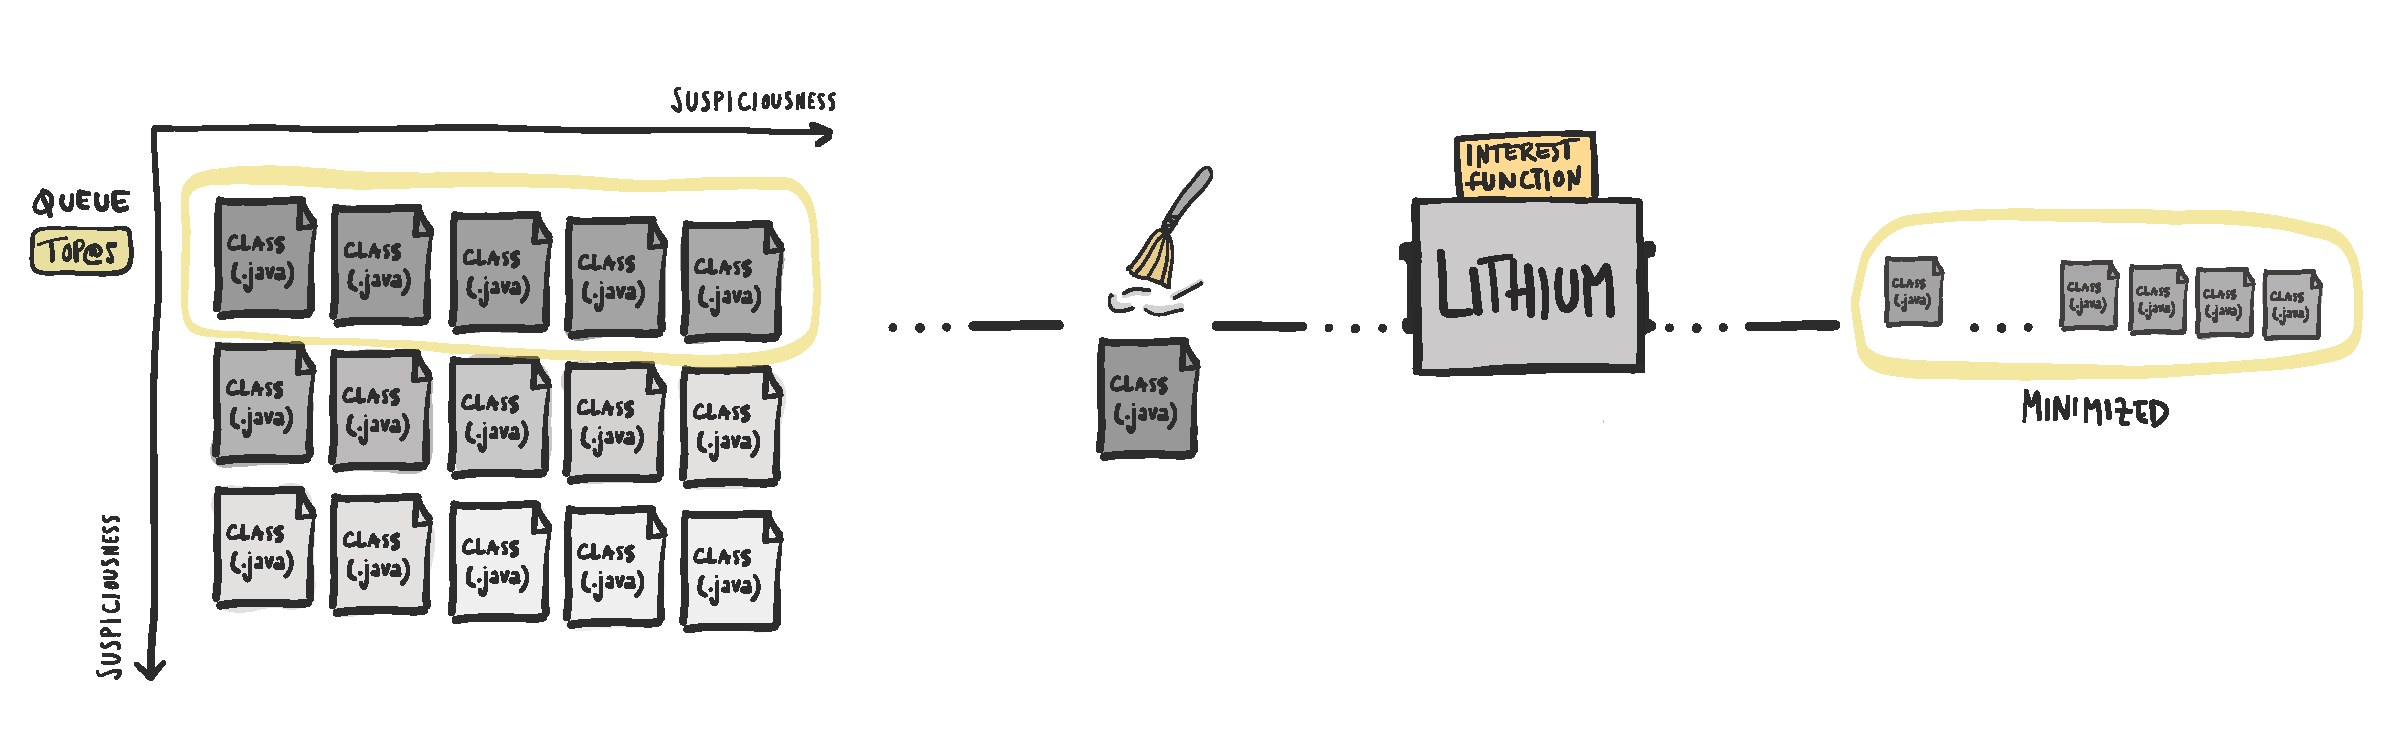
\includegraphics[width=1.0\textwidth]{lithium.pdf}
	\caption{Simple illustration of the process to obtain the top-5 minimized classes from a project carrying a bug}
\end{figure*}

\subsection{Function of Interest }
\label{sec:funcofint}


\begin{algorithm}[h]
	\caption{Function of interest (iFunc)}
	\label{alg:finc}
	\begin{flushleft}
		\textbf{Input:} $c$ - class to be minimized\\
		\hspace{2.75em} $t$ - testcase name\\
		\hspace{2.75em} $expStk$ -  expected stacktrace\\
		\textbf{Output:} $interest$ - $True$ if it is interesting, $False$ if not \\
	\end{flushleft}
	\begin{algorithmic}[1]
		\Function{iFunc}{$c$, $t$, $expStk$}
		\State $testStk \leftarrow$ runTest($t$)
		\State $testOracle \leftarrow$ getOracleToCompare($testStk$)
		\State $expOracle \leftarrow$ getOracleToCompare($expStk$)
		\State \Return $testOracle$ == $expOracle$
		\EndFunction

	\end{algorithmic}

\end{algorithm}

The \texttt{MozillaLithium} tool takes as input a function of interest that can be designed according to the problem to be solved. The function of interest (Algorithm \ref{alg:finc}) determines if the test case output is interesting or not. In this study, interesting means that the test execution path is equal to the expected one. This information can be deducted from \texttt{Java} stack traces which show the stack of functions called until the thrown of an exception. The authors assume that it is only necessary to compare both stack traces until the call where the test fails. For each chunk selected by \texttt{MozillaLithium}, the test is executed without considering the chunk under evaluation (Algorithm \ref{alg:finc}, line 2). Both test ($testStk$) and expected ($expStk$) stack traces are filtered according to the position of the test call fails. These operations are performed by line 3 and 4 from Algorithm 2. The result is an oracle such as the one provided in the box below:


\vspace{3mm}
\begin{myframe} \label{box:1}
java.lang.IndexOutOfBoundsException: Index: -1, Size: 1,
java.util.ArrayList.rangeCheckForAdd(ArrayList.java:643),
java.util.ArrayList.add(ArrayList.java:455),
org.jfree.data.xy.XYSeries.addOrUpdate(XYSeries.java:564),
org.jfree.data.xy.XYSeries.addOrUpdate(XYSeries.java:527),
\textbf{org.jfree.data.xy.junit.XYSeriesTests.}\\
\textbf{testBug1955483(XYSeriesTests.java:479)},\\
...
\end{myframe}

The oracle includes an exception error message (\emph{java.lang.\\IndexOutOfBoundsException: Index: -1, Size: 1}) and the program execution path until the class test where it fails (\emph{XYSeriesTests.java:479}). The regular expression \verb/Test(.*).java/ retrieves the test class position in the stack trace. If the test class is not found, the entire stack trace is compared. There is, however, an exception. When the failure is a \emph{StackOverflowError}, there is no test class mentioned in the stack trace because the exception is a runtime error. This exception is triggered when the JVM encounters a situation where there is no space for a new stack frame to be created which is, normally, the outcome of infinite recursion. Consequently, the stack trace contains many times the failed call. So, when the failure message contains a \emph{StackOverflowError}, the oracle is only considered until the call is repeated for the fifth time.

\vspace{3mm}
\begin{myframe}
	java.lang.StackOverflowError,
	sun.reflect.generics.reflectiveObjects.\linebreak
			TypeVariableImpl.hashCode(TypeVariableImpl.java:198),
	java.util.HashMap.hash(HashMap.java:362),
	java.util.HashMap.getEntry(HashMap.java:462),
	java.util.HashMap.get(HashMap.java:417),  org.mockito.internal.util.reflection.GenericMetadataSupport.
		getActualTypeArgumentFor(GenericMetadataSupport.java:182), \linebreak
	org.mockito.internal.util.reflection.GenericMetadataSupport.
	getActualTypeArgumentFor(GenericMetadataSupport.java:185),
	org.mockito.internal.util.reflection.GenericMetadataSupport.
	getActualTypeArgumentFor(GenericMetadataSupport.java:185),
	...
\end{myframe}

Some of the error messages can be different even if the test is executed with the same inputs and in the same environment. One example is the one provided in the box below, where the memory positions (\emph{class@<memory-position>}) may differ from the ones in the expected message. In order to solve this, it was designed a mechanism to check this kind of exception patterns. However, the current version of the interesting function only considers this pattern. Other patterns will be added soon into the next version of \lithium{}.

\vspace{3mm}
\begin{myframe}
	junit.framework.AssertionFailedError: \\
	expected:<org.jfree.chart.util.ShapeList@\textbf{d0e55451}> but \\ was:<org.jfree.chart.util.ShapeList@\textbf{d951b68f}>
	...
\end{myframe}



\section{Evaluation}
\label{sec:eval}

\Mar{-------------------- estou aqui}

This section reports results of our study to assess the impact of the
\comb{} combination.

\subsection{Objects of Analysis}

Following other recent studies, we used the \dfj{} benchmark in our
experiments~\cite{just-defects4j-issta2014}. The \dfj{} benchmark
includes six subjects and \numFaults{} faults.
\lang{} is a library
that provides a set of helper utilities for the {\small\texttt{java.lang}}
API. \cmath{} is a lightweight library of self-contained
mathematics and statistics components. The \closure{} is a toolset for
turning JavaScript files into smaller scripts for faster
download and execution in the browser. \chart{} is a library with a
full-featured charts user interface for Java. \jtime{} is a
lightweight library that aims to replace the default Java
{\small\texttt{java.util.Date}} classes providing simpler APIs. \mockito{} is
a mocking testing framework.\comments{ that enables the developer to simulate
the behavior of classes that cannot be used in unit testing.}

\newcommand{\cgray}[1]{\cellcolor{gray!25}#1}
\begin{table}[h]
  \centering
  \setlength{\tabcolsep}{4pt}
    \begin{tabular}{lrrr}
      \toprule
      Project            & Size (kLOC) & \# Tests & \# Defects \\ %\comments{& Failing Test Cases &}
      \midrule
      \lang{}            & 111751  & 6057 & 65       \\   %\commentst{& 124   &  -}\\
      \cmath{}           & 306276  & 26797 & 106     \\   %\comments{& 177   &  -}\\
      \closure{}         & 149521  & 27930  & 133     \\   %\comments{& 350   &  -}\\
      \chart{}           & 230159  & 8458 & 26      \\  %\comments{& 92    &  -}\\
      \jtime{}           & 141610  & 3289 & 27       \\   %\comments{& 76    &  -}\\
      \mockito{}         & 22787  & 8835 & 38    \\     %\comments{& 118   &  -}\\
      \bottomrule
  \end{tabular}
\caption {Characterization of \dfj{} subjects.}
\end{table}
\normalsize

%% old text related to single faults...
%%%%%%%%%%%%
%% It is important to note that the construction of the \dfj{} dataset is
%% not suited to evaluate the rate of single faults, but prior research
%% did that.  Perez~\etal{}~\cite{7927959} recently showed that single
%% faults are prevalent in open-source project. They conducted a
%% comprehensive empirical study involving 279 open-source Java projects
%% where they found that single faults were observed in 82\% of the cases
%% of regression.


\subsection{Results of Dynamic Slicing}

We describe the results of dynamic slicing alone in the following.


\Sof{@todo: after answering rqs add a subsection to discuss the performance of \ds{}}

\subsubsection{\textit{Does the critical slice include the faulty statements?}}



\subsubsection{\textit{How many test cases have the faulty statements in the top-5 of classes with the highest suspiciousness ranks?}}



\subsection{Results of \sfl{}+\ds{} Combination}

\subsubsection{\textit{How effective is the \sfl{}+\ds{} combination for bug localization?}}

\subsection{Threats to validity}

\pagebreak

%
%
%\subsubsection{How much reduction in one execution trace
%  can one get with Dynamic Slicing?}
%
%Table~\ref{fig:ds-reduction} shows the average reduction obtained with
%slicing considering our implementation. The first column shows the \dfj{} project name.
%Column ``Stmts. Covered'' shows the number of statements covered in
%the execution of one failing test, column ``Slice Size'' shows the
%number of statements appearing in the slice size, and column ``\%
%Reduction'' shows the percentage reduction obtained. Numbers reported
%are averaged across all executions. We only considered cases where we
%knew a priori the slice contained the faulty statements
%(Section~\ref{sec:ds-limitations}). Overall, it is noticeable that
%both absolute reduction (as per column ``Slice Size'') and relatitve
%reduction (as per column ``\% Reduction'') obtained are
%significant.
%
%\begin{table}[h]
%  \centering
%  %  \resizebox{\columnwidth}{!}{%
%  \setlength{\tabcolsep}{3pt}
%    \begin{tabular}{lrrrr}
%      \toprule
%      Project             & Stmts. & Slice &
%      \multicolumn{2}{c}{Reduction} \\
%      \cline{4-5}
%                          &  Covered &  Size  & \multicolumn{1}{c}{Avg.} & \multicolumn{1}{c}{$\sigma$}\\
%      \midrule
%      \lang{}             & 4,221             & 94            &  97.77\%  & -       \\
%      \cmath{}            & 743,587           & 175           &  90.16\%  & 14.98\% \\
%      \closure{}          & -                 & -             &  -        & -       \\
%      \chart{}            & 13,474            & 155           &  90.26\%  & 16.52\% \\
%      \jtime{}            & 23,360            & 912           &  95.99\%  & 01.25\% \\
%      \mockito{}          & 3,064             & 340           &  82.48\%  & 12.02\% \\
%      \bottomrule
%  \end{tabular}
%%}
%\caption {\label{fig:ds-reduction}Average reduction in slice sizes. We
%  rounded averages to the closest integer in columns
%  ``Stmts. Covered'' and ``Slice Size''.\Mar{Para a coluna
%    avg. reduction, o correto IMO eh tirar a media das reducoes e nao a
%    reducao media.  Mais precisamente, considerando lang, ao inves de
%    calcular 100*(4221-94)/4221 (como acima), deveriamos tirar a media
%das reducoes considerando cada caso de lang.}\Mar{Nao costumo ver
%    desvio padrao como percentagem}}
%\end{table}
%\normalsize
%
%\subsubsection{What are the limitations of Dynamic Slicing?}
%\label{sec:ds-limitations}
%
%%% Omission errors, implicit dependencies, and multiple regression faults
%%% can result in bug misses.  Omission errors occur when existing code
%%% requires no modification but new code is needed to fix a
%%% bug. Consequently, the slice of a failing test that manifests an
%%% omission error misses the faulty statements as they are yet to be
%%% added in code.  Figure~\Fix{ref} shows an example of omission
%%% error.\Mar{add example}\Mar{consider removing omission errors as
%%%   \sfl{} cannot handle this case anyway.  check what we did on ICST'17
%%%   paper.}
%
%%% \begin{figure}[h!]
%%%   \begin{lstlisting}[frame=single]  % Start your code-block
%%%     int myMethod(int myParam) {
%%%       var result: Int = 0
%%%       //result = myParam //This line is missing
%%%       if (myParam <= 10) {
%%%         result = result / 10
%%%       }
%%%       return result
%%%     }
%%%   \end{lstlisting}
%%%   \caption{\Luis{Exemplo de falha de omissao do tipo \textbf{New Code}}}
%%%   \label{example-new-code}
%%% \end{figure}
%
%The pie chart in Figure~\ref{pie-chart} highlights the sources of
%problems associated with slicing.  We classify the slicing task as
%problematic when it misses the faulty statement. A number of reasons
%can explain a miss:
%
%\begin{itemize}
%\item \textbf{Missing code:} this case happens when the
%bug is due to missing code. Any fault localization method, including
%Slicing and \sfl{}, are innefective in this case. This is the main
%source of problem we found in our dataset. Note that, although this
%problem is not specific to slicing, executable slices could be used to
%help the developer identify missing statements with
%inspection.
%
%\item \textbf{Non-observable effect:} This case happens when the
%buggy code does not produce effect on the output. Consider, for
%example, the scenario where there is a bug in a branch predicate that
%results in execution not taking the branch guarded by a
%conditional. In that case, the \CS{} is able to produce a slice that
%does not contain the faulty if statement, still reproducing the
%original output. This problem is specific to \CS{}. Note from the
%piechart that this is the second most prevalent source of problem but
%much less significant compared to missing
%code.
%
%\item \textbf{Non-deterministic output:} This case happens when the
%  output of the program changes in every execution, such as random
%  output sizes. Although, we handled specific cases such as that of a
%  hashcode printed on the stack trace, which we are able to detect
%  with re-execution, in general, \CS{} cannot pinpoint those cases.
%  Consider, for example, the case of a stack overflow where the trace
%  can vary from one execution to another.
%
%%% There are supported cases, such as small changes in the output (i.e.,
%%% hashcode of an object printed in the stack trace). Although,
%%% StackOverflowException is not one of those cases, which the size of
%%% lines printed is not the same.
%
%\end{itemize}
%
%
%\begin{figure}[ht]
%  \centering
%  \begin {tikzpicture}
%    \pie[
%      text=pin,
%      radius=1.5,
%      color={
%        white!22.1,
%        white!14.7,
%        white!1.6,
%        white!61.6
%      }
%    ]{
%      61.6/{Missing Code (117)},
%      14.7/{Non-Observable Effect (28)},
%      1.6/{Non-deterministic Output (3)},
%      22.1/{REMOVEME (42)}
%    }
%  \end {tikzpicture}
%  \caption{\label{pie-chart}Source of problems in \Fix{XX} of the
%    \Fix{YY} cases where Dynamic Slicing misses the faulty statement.}
%\end{figure}
%
%\Fix{I was left wondering: so what? What is the message and the actionable points?}
%\Fix{The goal of this paper is debugging, so we should answer the question: does
%dynamic slicing alone help in debugging?}
%
%\subsection{Results of the \comb{} combination}
%
%This section describes the results of the \comb{} combination. The
%independent variables we used in the following experiments are (i) the
%selection of tests to slice (see Section~\ref{sec:combination}) and
%(ii) whether ot not the statements covered by selected tests are
%filtered from the ranking.  Considering the first variable, the
%illustration above shows the effect of slicing code using a single
%failing test. However, we also analyzed the combination where we
%compute slices of all failing tests. Intuitively, in those cases, more
%lines in the matrix would be affected. The rationale for varying the
%selection of tests to slice is to assess the impact that the amount of
%slicing code has on performance of \sfl{}.  Considering the second
%variable, the illustration above shows the scenario where all
%components are reported in the ranking. However, we also analyzed the
%scenario where only the components covered by our selection of tests
%appear in the ranking. For the case above, only $c_2$ and $c_5$ would
%be listed.  The dependent variable we used was the performance of
%\sfl{} measured with
%Top@N~\cite{Wu:2014:CLC:2610384.2610386,Lucia:2014:FFL:2642937.2642983,Wen:2016:LLB:2970276.2970359},
%which indicates, for a given value N, the percentage of faults ranked
%at position no lower than N. As recently discussed by Ang
%\etal~\cite{ang-perez-van-deursen-rui-2017}, \sfl{} researchers
%started using absolute metrics, such as Top@N, after Parnin and
%Orso~\cite{parnin-orso-2011} highlighed the bias in metrics based on
%the position of the faulty statement in the ranking relative to the
%total size of the ranking, which is often very high. It is worth
%mentioning that we used the GZoltar~\cite{gzoltar} toolset to run our
%experiments.
%
%\Fix{discutir Tabela~\ref{tab:summary}...}
%
%
%\begin{table}[h]
%  \centering
%  \setlength{\tabcolsep}{4pt}
%    \begin{tabular}{lrrrr}
%      \toprule
%      Project            & (1,N) & (1,F) & (A,N) & (A,F)  \\
%      \midrule
%      \lang{}            & -  & - & -  & - \\
%      \cmath{}           & -  & - & -  & - \\
%      \closure{}         & -  & - & -  & - \\
%      \chart{}           & -  & - & -  & - \\
%      \jtime{}           & -  & - & -  & - \\
%      \mockito{}         & -  & - & -  & - \\
%      \bottomrule
%  \end{tabular}
%\caption {\label{tab:summary}Summary of results considering Top@N, for
%  N=50, which is the midpoint value of N for the range we selected
%  1-100.}
%\end{table}
%\normalsize
%
%\subsubsection{What is the impact of slicing one failing test?}
%This scenario reflects the case where the developer selects one given
%test to focus debugging efforts. Figure \ref{fig:one-failing-test}
%compares the results of \sfl{} and \comb{} when slicing code
%associated with a single failing test. The top section of the figure
%shows results without filtering covered statements whereas the lower
%section shows the results with filtering. Each table shows the results of \sfl{} and \comb{}
%for increasing values of N.  The top section of each table shows the
%results for \sfl{} whereas the lower section shows results of
%\comb{}. A plot for each subject appears under the tables to
%illustrate how techniques compare. The x-axis denote the value of N
%and the y-axis denotes the value of Top@N. Informally, a quick
%increase is good~--~it means a high percentage of faults was detected
%for small values of N.\Mar{@Rui, ainda nao esta claro qual a mensagem
%  que vamos transmitir. Considerando resultados atuais, existe
%  reducao, mas parece ser pouca para N<20. Existe algum valor de N
%  considerado referencia para que a gente possa dar mais substancia ao
%  resultado?}
%
%\subsubsection{What is the impact of slicing all failing tests?}
%Table~\ref{fig:all-failing-tests} \Fix{...............}

%
%\begin{figure*}[!ht]
%  \centering
%    \begin{tabular}{cl|rrrrrrrrrr}
%      \toprule
%      & \multicolumn{1}{c|}{Project~\textbackslash{}~LOC}             & 10  & 20  & 30  &  40  & 50  & 60 & 70 &  80 &  90& 100 \\
%      \midrule
%
%      \multicolumn{12}{c}{\emph{\textbf{Not} Filtering statements covered by test(s).}}\\
%      \midrule
%      \parbox[t]{2mm}{\multirow{4}{*}{\rotatebox[origin=c]{90}{\footnotesize{\sfl}}}}
%      & \lang{}       & 24.72 & 25.84 & 28.09 & 32.58 & 35.96 & 46.07 & 79.78 & 79.78 & 83.15 & 84.27 \\
%      & \chart{}      & 18.97 & 24.14 & 31.03 & 31.03 & 32.76 & 72.41 & 72.41 & 75.86 & 79.31 & 79.31 \\
%      & \jtime{}      & 34.78 & 58.7  & 63.04 & 63.04 & 63.04 & 63.04 & 63.04 & 63.04 & 71.74 & 71.74 \\
%      & \mockito{}    & 44.32 & 47.73 & 57.95 & 61.36 & 61.36 & 63.64 & 65.91 & 70.45 & 76.14 & 77.27 \\
%      \hline
%      \parbox[t]{2mm}{\multirow{4}{*}{\rotatebox[origin=c]{90}{\footnotesize{\comb}}}}
%      & \lang{}       & 31.46 & 37.08 & 51.69 & 57.3  & 65.17 & 77.53 & 80.9  & 82.02 & 87.64 & 91.01 \\
%      & \chart{}      & 43.1  & 46.55 & 60.34 & 81.03 & 94.83 & 96.55 & 96.55 & 96.55 & 96.55 & 98.28 \\
%      & \jtime{}      & 50.0  & 63.04 & 63.04 & 63.04 & 63.04 & 67.39 & 71.74 & 71.74 & 71.74 & 71.74 \\
%      & \mockito{}    & 45.45 & 47.73 & 60.23 & 60.23 & 61.36 & 62.5  & 67.05 & 76.14 & 79.55 & 80.68 \\
%      \midrule
%
%      \multicolumn{2}{c}{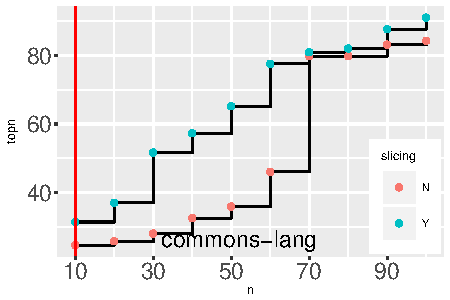
\includegraphics[width=0.25\textwidth]{R/commons-lang-onefailingtest.pdf}}
%      &
%      \multicolumn{5}{c}{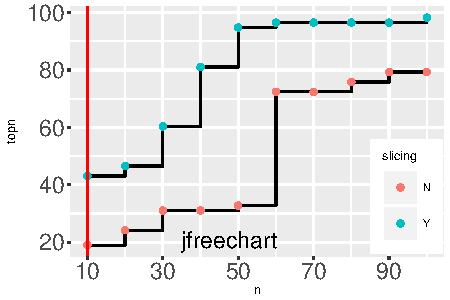
\includegraphics[width=0.25\textwidth]{R/jfreechart-onefailingtest.pdf}}
%      &
%      \multicolumn{5}{c}{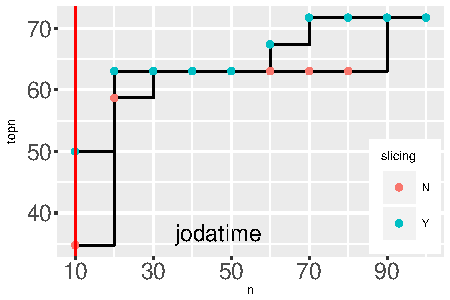
\includegraphics[width=0.25\textwidth]{R/jodatime-onefailingtest.pdf}}\\
%
%      \multicolumn{2}{c}{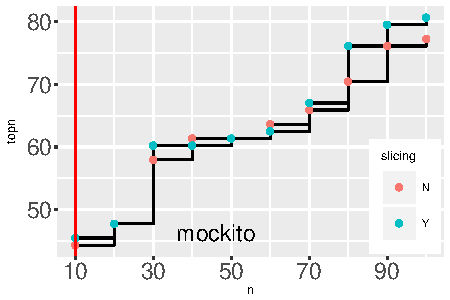
\includegraphics[width=0.25\textwidth]{R/mockito-onefailingtest.pdf}}
%      &
%      \multicolumn{5}{c}{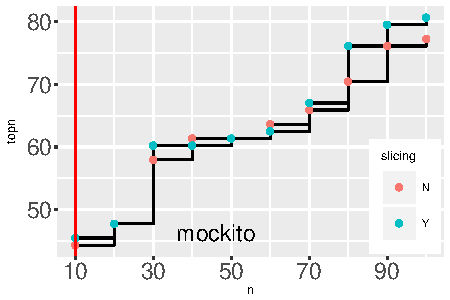
\includegraphics[width=0.25\textwidth]{R/mockito-onefailingtest.pdf}}
%      &
%      \multicolumn{5}{c}{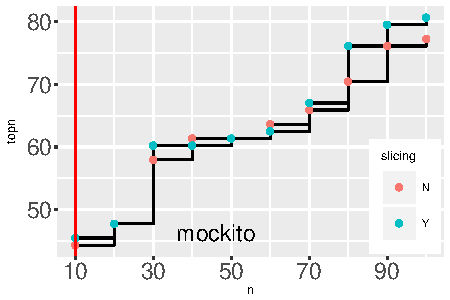
\includegraphics[width=0.25\textwidth]{R/mockito-onefailingtest.pdf}}\\
%
%      \midrule
%
%      \multicolumn{12}{c}{\emph{Filtering statements covered by test(s).}}\\
%      \midrule
%      \parbox[t]{2mm}{\multirow{4}{*}{\rotatebox[origin=c]{90}{\footnotesize{\sfl}}}}
%      & \lang{}     & 33.71 & 41.57 & 49.44 & 52.81 & 60.67 & 84.27 & 94.38 & 95.51 & 96.63 & 98.88 \\
%      & \chart{}    & 25.86& 36.21& 36.21& 36.21& 60.34& 75.86& 75.86 & 79.31& 79.31& 79.31 \\
%      & \jtime{}       & 43.48 & 63.04 & 65.22 & 69.57 & 71.74 & 71.74 &73.91 & 73.91 & 73.91 & 73.91 \\
%      & \mockito{} & 72.09 & 74.42 & 77.91 & 80.23 & 83.72 & 83.72 & 84.88 & 84.88 & 86.05 & 86.05 \\
%      \midrule
%      \parbox[t]{2mm}{\multirow{4}{*}{\rotatebox[origin=c]{90}{\footnotesize{\comb}}}}
%      & \lang{}     & 46.07 & 58.43 & 66.29 & 67.42 & 74.16 & 93.26 & 97.75 & 98.88 & 100.0 & 100.0 \\
%      & \chart{} & 51.72& 63.79& 65.52& 86.21& 98.28& 98.28& 98.28& 98.28& 98.28& 98.28 \\
%      & \jtime{} & 65.22 & 69.57 & 73.91 & 73.91 & 73.91 & 73.91 & 73.91 & 73.91 & 73.91 & 73.91 \\
%      & \mockito{} & 73.26 & 77.91 & 82.56 & 87.21 & 87.21 & 88.37 &91.86 & 94.19 & 95.35 & 95.35 \\
%      \midrule
%
%      \multicolumn{2}{c}{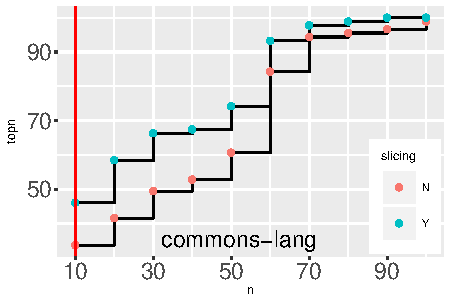
\includegraphics[width=0.25\textwidth]{R/commons-lang-onefailingtest-filtering.pdf}}
%      &
%      \multicolumn{5}{c}{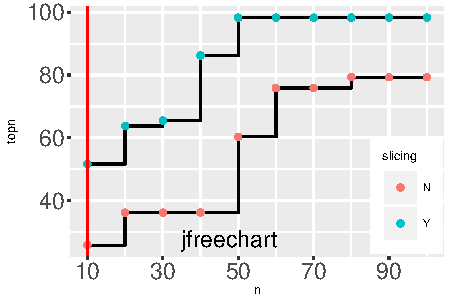
\includegraphics[width=0.25\textwidth]{R/jfreechart-onefailingtest-filtering.pdf}}
%      &
%      \multicolumn{5}{c}{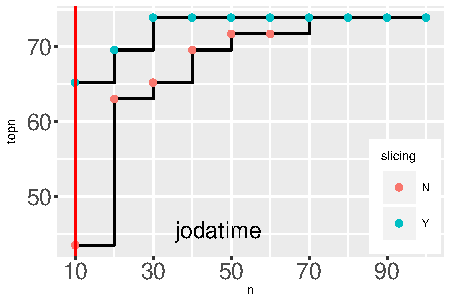
\includegraphics[width=0.25\textwidth]{R/jodatime-onefailingtest-filtering.pdf}}\\
%
%      \multicolumn{2}{c}{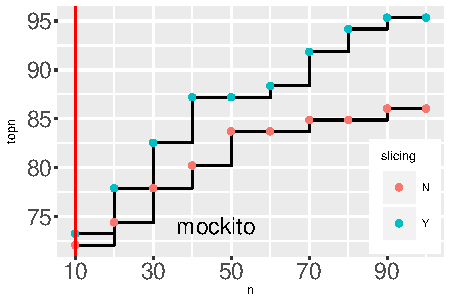
\includegraphics[width=0.25\textwidth]{R/mockito-onefailingtest-filtering.pdf}}
%      &
%      \multicolumn{5}{c}{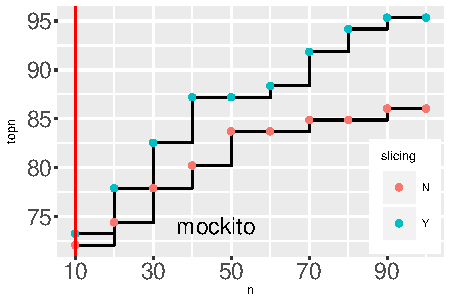
\includegraphics[width=0.25\textwidth]{R/mockito-onefailingtest-filtering.pdf}}
%      &
%      \multicolumn{5}{c}{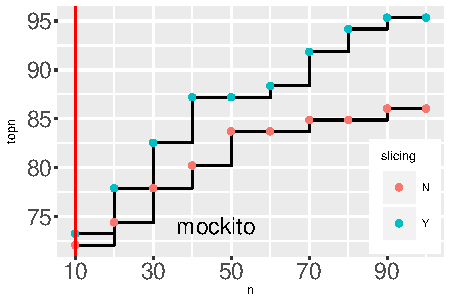
\includegraphics[width=0.25\textwidth]{R/mockito-onefailingtest-filtering.pdf}}\\
%
%      \bottomrule
%
%    \end{tabular}
%    \caption{\label{fig:one-failing-test}Top@N, considering one failing test.}
%\end{figure*}
%
%\begin{figure*}[!ht]
%  \centering
%    \begin{tabular}{cl|rrrrrrrrrr}
%      \toprule
%      & \multicolumn{1}{c|}{Project~\textbackslash{}~LOC}             & 10  & 20  & 30  &  40  & 50  & 60 & 70 &  80 &  90& 100 \\
%      \midrule
%
%      \multicolumn{12}{c}{\emph{\textbf{Not} Filtering statements covered by test(s).}}\\
%      \midrule
%      \parbox[t]{2mm}{\multirow{4}{*}{\rotatebox[origin=c]{90}{\sfl}}}
%      &Apache commons-lang     & 25.0  & 27.27 & 29.55 & 38.64 & 43.18
%      & 56.82 & 63.64 & 63.64 & 68.18 & 70.45 \\
%      &\chart{}       & 50.0  & 68.75 & 75.0  & 75.0  & 75.0  & 87.5  & 87.5  & 87.5  & 93.75 & 93.75 \\
%      &Joda-Time       & 23.08 & 38.46 & 46.15 & 46.15 & 46.15 & 46.15
%      & 46.15 & 46.15 & 46.15 & 46.15 \\
%      &Mockito & 16.67 & 29.17 & 33.33 & 37.5  & 37.5  & 41.67 & 45.83
%      & 54.17 & 58.33 & 62.5 \\
%      \hline
%      \parbox[t]{2mm}{\multirow{4}{*}{\rotatebox[origin=c]{90}{\comb}}}
%      &Apache commons-lang     & 36.36 & 50.0  & 56.82 & 59.09 & 63.64
%      & 65.91 & 65.91 & 68.18 & 75.0  & 81.82 \\
%      & \chart{}       & 68.75 & 81.25 & 93.75 & 100.0 & 100.0 & 100.0 & 100.0 & 100.0 & 100.0 & 100.0 \\
%      &Joda-Time       & 30.77 & 46.15 & 46.15 & 46.15 & 46.15 & 46.15
%      & 46.15 & 46.15 & 46.15 & 46.15 \\
%      &Mockito & 20.83 & 29.17 & 41.67 & 41.67 & 41.67 & 45.83 & 58.33
%      & 66.67 & 70.83 & 75.0 \\
%      \midrule
%
%      \multicolumn{2}{c}{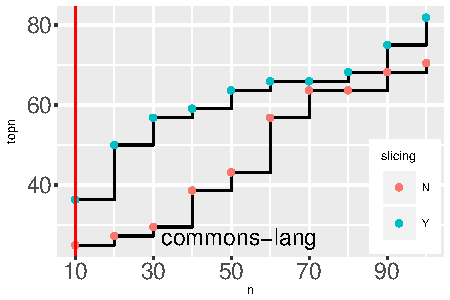
\includegraphics[width=0.25\textwidth]{R/commons-lang-allfailingtest.pdf}}
%      &
%      \multicolumn{5}{c}{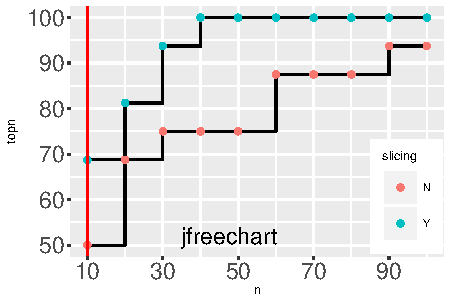
\includegraphics[width=0.25\textwidth]{R/jfreechart-allfailingtest.pdf}}
%      &
%      \multicolumn{5}{c}{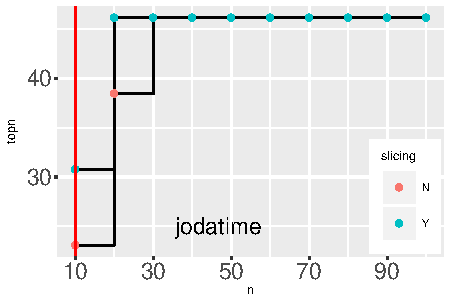
\includegraphics[width=0.25\textwidth]{R/jodatime-allfailingtest.pdf}}\\
%
%      \multicolumn{2}{c}{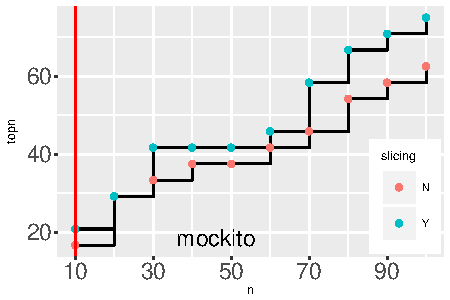
\includegraphics[width=0.25\textwidth]{R/mockito-allfailingtest.pdf}}
%      &
%      \multicolumn{5}{c}{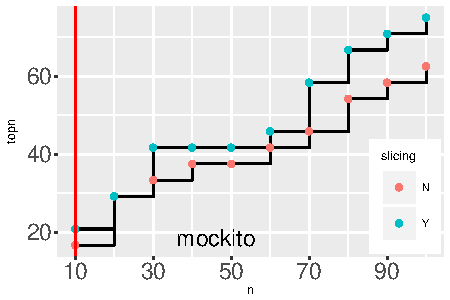
\includegraphics[width=0.25\textwidth]{R/mockito-allfailingtest.pdf}}
%      &
%      \multicolumn{5}{c}{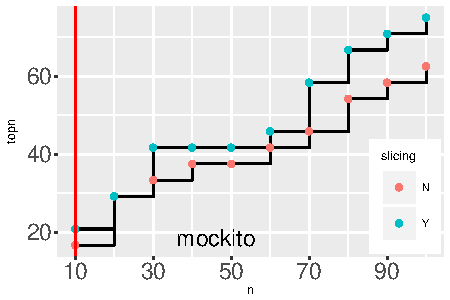
\includegraphics[width=0.25\textwidth]{R/mockito-allfailingtest.pdf}}\\
%      \midrule
%
%      \multicolumn{12}{c}{\emph{Filtering statements covered by test(s).}}\\
%      \midrule
%      \parbox[t]{2mm}{\multirow{4}{*}{\rotatebox[origin=c]{90}{\footnotesize{\sfl}}}}
%      & \lang{}     & 36.36 & 45.45 & 59.09 & 63.64 & 70.45  & 79.55 & 88.64 & 90.91 & 93.18 & 97.73 \\
%      & \chart{}       & 50.0  & 68.75 & 75.0  & 75.0  & 75.0  & 87.5  & 87.5  & 93.75 & 93.75 & 93.75 \\
%      & \jtime{}        & 30.77 & 46.15 & 46.15 & 46.15 & 46.15 & 46.15  & 53.85 & 53.85 & 53.85 & 53.85 \\
%      & \mockito{} & 50.0  & 54.17 & 62.5  & 66.67 & 70.83 & 75.0  & 79.17 & 79.17 & 79.17 & 79.17 \\
%      \hline
%      \parbox[t]{2mm}{\multirow{4}{*}{\rotatebox[origin=c]{90}{\footnotesize{\comb}}}}
%      & \lang{}     & 56.82 & 81.82 & 93.18 & 93.18 & 95.45  & 95.45 &95.45 & 97.73 & 100.0 & 100.0 \\
%      & \chart{}       & 68.75 & 87.5  & 93.75 & 100.0 & 100.0 & 100.0 & 100.0 & 100.0 & 100.0 & 100.0 \\
%      & \jtime{}        & 53.85 & 53.85 & 53.85 & 53.85 & 53.85 & 53.85  & 53.85 & 53.85 & 53.85 & 53.85 \\
%      & \mockito{} & 54.17 & 70.83 & 79.17 & 83.33 & 83.33 & 87.5  & 87.5 & 87.5  & 91.67 & 91.67 \\
%      \midrule
%
%      \multicolumn{2}{c}{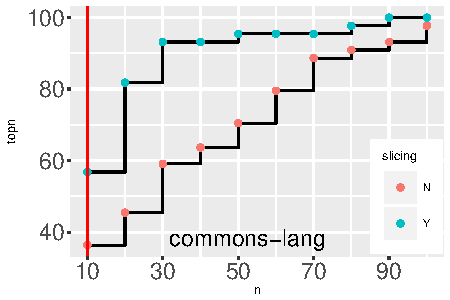
\includegraphics[width=0.25\textwidth]{R/commons-lang-allfailingtest-filtering.pdf}}
%      &
%      \multicolumn{5}{c}{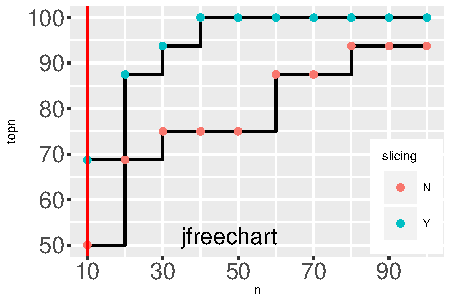
\includegraphics[width=0.25\textwidth]{R/jfreechart-allfailingtest-filtering.pdf}}
%      &
%      \multicolumn{5}{c}{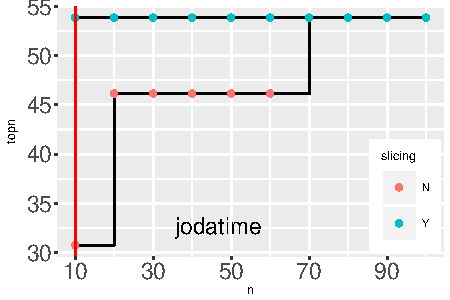
\includegraphics[width=0.25\textwidth]{R/jodatime-allfailingtest-filtering.pdf}}\\
%
%      \multicolumn{2}{c}{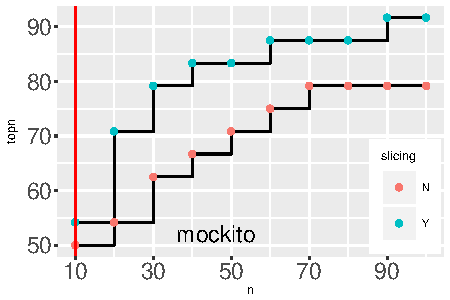
\includegraphics[width=0.25\textwidth]{R/mockito-allfailingtest-filtering.pdf}}
%      &
%      \multicolumn{5}{c}{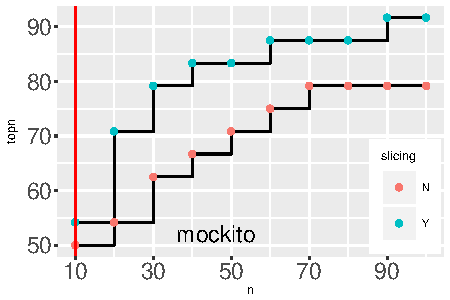
\includegraphics[width=0.25\textwidth]{R/mockito-allfailingtest-filtering.pdf}}
%      &
%      \multicolumn{5}{c}{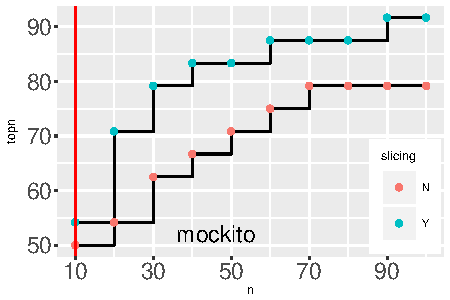
\includegraphics[width=0.25\textwidth]{R/mockito-allfailingtest-filtering.pdf}}\\
%      \bottomrule
%
%    \end{tabular}
%    \caption{\label{fig:all-failing-test}Top@N, considering all failing test.}
%\end{figure*}


%
%We pose the following research questions:

%\textit{RQ1: How frequent are dynamic slices without the bug produced? }
%~\Davino{ XX\% of the results show omission cases, i.e., cases where the fault of the program wasn't present on the generated slice. }

%\textit{RQ2: Are SFL techniques effective on minimizing the effort to manual/automated fault localization?}
%~\Davino{ With the results, we show that it surely isn't. Rank of
%suspiciousness commonly puts the fault at the top 50+ lines of code,
%which isn't practical using manual or automated fault localization, or
%even automated program repair.}

%\textit{RQ3: Can Critical Slicing improve Statistical Fault Localization of real faults in a program?}
%~\Davino{ The results are based on REAL faults (instead of artificial
%ones, which are the basis case of evaluations of techniques involving
%slicing and SFL) presented in Defect4J's data set and show small
%improvements when comparing SFL and DS+SFL.}

\section{Related Work}


\subsection{Program Slicing}

Program Slicing is an old technique with several applications in PL
and SE research~\cite{Weiser:1981:PS:800078.802557}. Slicing can be
implemented in different ways. Dynamic Slicing has found its main
application in fault
localization~\cite{Agrawal:1990:DPS:93542.93576}---in this application
context, failing tests exist. Research in this area has mainly focused
on slicing code
efficiently~\cite{Wang:2008:DSJ:1330017.1330021,Wang:2004:UCB:998675.999455}
and avoiding data and control omission
errors~\cite{Zhang:2007:TLE:1250734.1250782,
  Lin:2018:BDE:3238147.3238163}. Omission errors correspond to the
cases where tests fail because some part of the code was not executed
when it should. Dynamic fault localization techniques cannot hope to
soundly report bugs in those cases. The issue is that incorporating
static information to capture those cases can result in unacceptably
large slices, which defeats the purpose of reducing the fault search
space. It is worth noting that, conceptually, the \comb{} combination
can be used with any form of dynamic slicing. We chose an
implementation of Critical
Slicing~\cite{DeMillo:1996:CSS:229000.226310} for its generality.

%% ORBS~\cite{Binkley:2014:OLP:2635868.2635893,DBLP:conf/iwpc/IslamB16}
%% is a recently-proposed slicing technique that is similar to Critical
%% Slicing. It is worth noting that


\subsection{SFL}

Statistics-based techniques (e.g.,~\cite{Pearson:2017:EIF:3097368.3097441}) are
popular automated fault localization techniques within the Software Engineering
community. They correlate information about program fragments that have been
exercised in multiple program execution traces (also called \textit{program
spectra}) with information about successful and failing executions. By doing
that, statistics-based approaches yield a list of suspect program fragments
sorted by their likelihood to be at fault. Since this technique is efficient in
practice, it is attractive for large modern software systems~\cite{ecbs07}.

Spectrum-based fault localization (\sfl) is amongst the most common statistical
fault localization technique that takes as input a test suite including at least
one failing test and reports on output a ranked list of components likely to be
in fault~\cite{FLSurvey2016, DBLP:conf/kbse/JonesH05,
DBLP:journals/smr/LuciaLJTB14, DBLP:journals/jss/AbreuZGG09}.

\subsection{\comb{}}

Prior work has investigated the combination of dynamic slicing and
spectrum-based fault
localization~\cite{Wotawa:2010:FLB:1848650.1849235,Alves:2011:FUD:2190078.2190115,DBLP:conf/ecai/HoferW12,lei-mao-dai-wang-2012,slicing-sfl-repair}. Although
the methodology used in these papers vary, the overall message is that
the combination is valuable. Note that slicing alone does not provide
the guarantee of improvement to \sfl{} as statements discarded with
slicing could have been ranked lower compared to faulty
statements. This paper differs from prior work in that it uses a much
larger dataset of programs and faults and a more rigorous experimental
methodology.


\subsubsection{Applications}

Ishii and Kutsuna ~\cite{li-huo-chen-zhong-feng-li-2013} proposed a
technique involving dynamic slicing and SFL applied to MATLAB/Simulink
models. The technique consists of iteratively
generating tests that cause an error using satisfiability modulo
theories (SMT) so that the slices generated are distinct from each
other.  For slicing, their technique uses a program dependence graph
(PDG) that express both data and control dependencies between blocks,
so that the slice is built only on blocks that affect a specific line
in the model - \textit{effective blocks}.  Their goal with the slicing
was (1) to keep suspiciousness of a fault maximum if a target model
has only one fault, and (2), to reduce the number of fault candidates
obtained by the slicer.  For this, they utilize only failed test cases
generated with SMT solvers ~\cite{peleska-vorobev-lapschies-2011} to
calculate suspiciousness, as passed test cases might lower the
suspiciousness of a fault.  The calculated suspiciousness is the
number of times that a block belongs to the \textit{effective blocks}
group by the number of total failed test cases.  Although their
experiments and results showed promise with small models, the accuracy
of the technique decreases when applied to models with multiple faults
instead of one, as does the efficiency when exposed to large models,
number of generated tests, sizes of sliced models and so on.

\subsubsection{Automatic Program Repair}
Automated repair techiniques have received considerable attention on
the last decade and consists of three basic steps: fault localization, patch
generation, and patch validation.  Regarding the fault localization
step, Automated Program Repair (APR) tools can be guided by statistical
fault localization techiniques to modify code which most likely
contains the fault. On this section, we will briefly describe some of
these tools.
\Davino { Not necessarily on the paper and not necessarily on a related work section. To be revised/moved/sliced later. }

GenProg\Fix{cite} is a state of the art tool based on genetic
programming to repair defects in off-the-shelf C programs. GenProg's
strategy to fault localization consists of instrumenting the program
so that all lines visited when executing failing test cases are
recorded and used on the genetic search algorithm. The algorithm
involves serching for other parts of the program, considering that a
program that contains an error in one area likely implements the
correct behaviour elsewhere. The tool proved to be effective in
reparing 16 programs involving 1.25 millions LOC, and efficient as the
algorithm search space takes advantage of test case coverage
information, reusing  existing program statements.

Debroy and Wong\Fix{cite} presented a techinique for automatically
fixing faults in a program combining both mutation and statistical
fault localization. Using the Tarantula fault localizer\Fix{cite}, the
techinique focus the top ranked statements in terms of suspiciousness
for the mutation operations. The percentage of statements examined in
search for the fault is based on the total number of statements of the
program, with the 10 percent being a reasonable number on the subject
programs studied.

JAFF\Fix{cite} is a Java automatic repair tool based on evolutionary principles that uses fault localization for ranking the statements in the code in terms of suspiciousness level.
Before searching for the fix, the Java program is translated into a syntax tree composed of nodes related to the top ranked statements being used on the search process.
The tool uses a specific formula to get the number of nodes that will be used on the search based on the number of statements with the same rank of suspiciousness,
with the range between 1 to 20 nodes being used on the cases studied.

SemFix is based on symbolic execution, constraint solving and program synthesis applied to software automatic repair. The tool uses statistical fault localization (SFL) with Tarantula to
obtain the rank of suspiciousness and iteratively takes the most suspicious statement that has not been tried out to be used on the search for a fix. Compared to GenProg, the presented tool
took consideredably less time to find a fix for programs utilizing the same test suites. However, the authors mention that the choice of the SFL techinique could potentially affect the
effectiviness of the tool, particularly with large programs.

SPR\Fix{cite} \Davino{ Fan Long } is based on staged
program repair with condition synthesis. SPR uses fault localization
to identify target statements that will be transformed in search for a
fix on the program. The search space is built with a list of
statements ranked by suspiciousness level, where only the first 200
ranked statements are considered. The authors observed that increasing
the search space to the top 2000 statements would bring additional
repairs, but with a obvious cost of searching a large space.
\Davino { Another tool presented by the same authors is Prophet, which uses the same search space, top 200. }

MintHint \Fix{cite} uses statistical analysis with SFL to rank
statements by their likelihood of being faulty. Given the ranked list,
the tool analysis the top \textit{k} statements, where \textit{k} is a
threshold set by the user, and proceeds with the repair algorithm
assuming the fault can be repaired by changing a single statement.


\Davino { Another set of automatic program repair tools that doesn't use fault localization includes: CodePhage, ClearView, PAR, RSRepair, Kali, and AutoFix, among others. }




\section{Conclusions and Future Work}\label{sec:conc}

%% Acknowledgments
\begin{acks}                            %% acks environment is optional

  %% Commands \grantsponsor{<sponsorID>}{<name>}{<url>} and
  %% \grantnum[<url>]{<sponsorID>}{<number>} should be used to
  %% acknowledge financial support and will be used by metadata
  %% extraction tools.
  This material is based upon work supported by the
  \grantsponsor{GS100000001}{National Science
    Foundation}{http://dx.doi.org/10.13039/100000001} under Grant
  No.~\grantnum{GS100000001}{nnnnnnn} and Grant
  No.~\grantnum{GS100000001}{mmmmmmm}.  Any opinions, findings, and
  conclusions or recommendations expressed in this material are those
  of the author and do not necessarily reflect the views of the
  National Science Foundation.
\end{acks}

%% Bibliography
\bibliography{tmp}

%% Appendix
%% \appendix
%% \section{Appendix}
%% Text of appendix \ldots

\end{document}
